\documentclass[midterm]{sparreport}

\title{Non-Ergodic Mess3: Belief State Geometry with Multiple Components}

\author{
  \textbf{Elena Ajayi}\\
  \texttt{elenaajayi@example.com}
}

\sparround{Spring 2025}

\begin{document}

\maketitle

\begin{abstract}
% YOUR ABSTRACT HERE (100-200 words)
\end{abstract}

\keywords{belief state geometry \and mechanistic interpretability \and
  non-ergodic mixtures \and hidden Markov models}

% ------------------------------------------------------------------
\section{Why Non-Ergodic Structure Matters}

% YOUR WRITING HERE

% ------------------------------------------------------------------
\section{Setup}

% YOUR WRITING HERE
% Key numbers for reference:
% - 3 components: alpha = 0.4, 0.7, 0.9, shared x = 0.1
% - Sequence length: 16, component identity hidden
% - Transformer: 3 layers, 2 heads, d_model=64, 152K params
% - Training: 15K steps, Adam lr=1e-3, cosine schedule
% - Final loss: 0.994 (uniform entropy = ln(3) = 1.099)

% ------------------------------------------------------------------
\section{Pre-Registered Predictions}

% YOUR WRITING HERE
% Predictions:
% 1. Shared subspace, not orthogonal (cite factoredrepresentations2025)
% 2. Both jobs compound across layers (cite constrainedbelief2025)
% 3. Gradual context separation (cite riechers2025)
% 4. Sharp training transition (cite olsson2022)
% 5. Final layer sufficient
%
% Math: belief update eta' = eta * T[token] / Z is piecewise-linear

% ------------------------------------------------------------------
\section{Results}

% YOUR WRITING HERE
% Key numbers:
%
% Prediction 1 (CONFIRMED):
%   Effective dim = 6, top 5 PCs = 94.5% variance
%   Subspace overlap: 0.4v0.7 = 0.992, 0.4v0.9 = 0.967, 0.7v0.9 = 0.990
%
% Prediction 2 (PARTIAL):
%   emb:     R2=0.643, Acc=0.333, Sil=-0.007
%   layer_0: R2=0.810, Acc=0.455, Sil=-0.019
%   layer_1: R2=0.847, Acc=0.519, Sil=+0.009
%   layer_2: R2=0.840, Acc=0.527, Sil=-0.008
%   ln_f:    R2=0.842, Acc=0.523, Sil=-0.042
%
% Prediction 3 (REFUTED):
%   Silhouette negative at every position (-0.22 at pos 0, ~-0.03 elsewhere)
%
% Prediction 4 (REFUTED):
%   Silhouette ~-0.04 throughout training, no phase transition
%   R2 rises 0.75 -> 0.83 by step 1000, then plateaus
%
% Prediction 5 (CONFIRMED):
%   Final layer R2 = 0.849, all-layers R2 = 0.853, gap = 0.005

% Summary table you can use:
\begin{table}[htbp]
  \centering
  \begin{tabular}{llc}
    \toprule
    Prediction & Key Result & Confirmed? \\
    \midrule
    1. Shared subspace & Overlap 0.97--0.99 & Yes \\
    2. Compounding layers & $R^2$ rises, silhouette does not & Partial \\
    3. Gradual separation & Silhouette $\approx -0.03$ everywhere & No \\
    4. Sharp transition & No jump across training & No \\
    5. Final layer sufficient & $R^2$ gap $= 0.005$ & Yes \\
    \bottomrule
  \end{tabular}
\end{table}

% Figures — uncomment once PNGs are in figures/ directory
\begin{figure}[htbp]
  \centering
  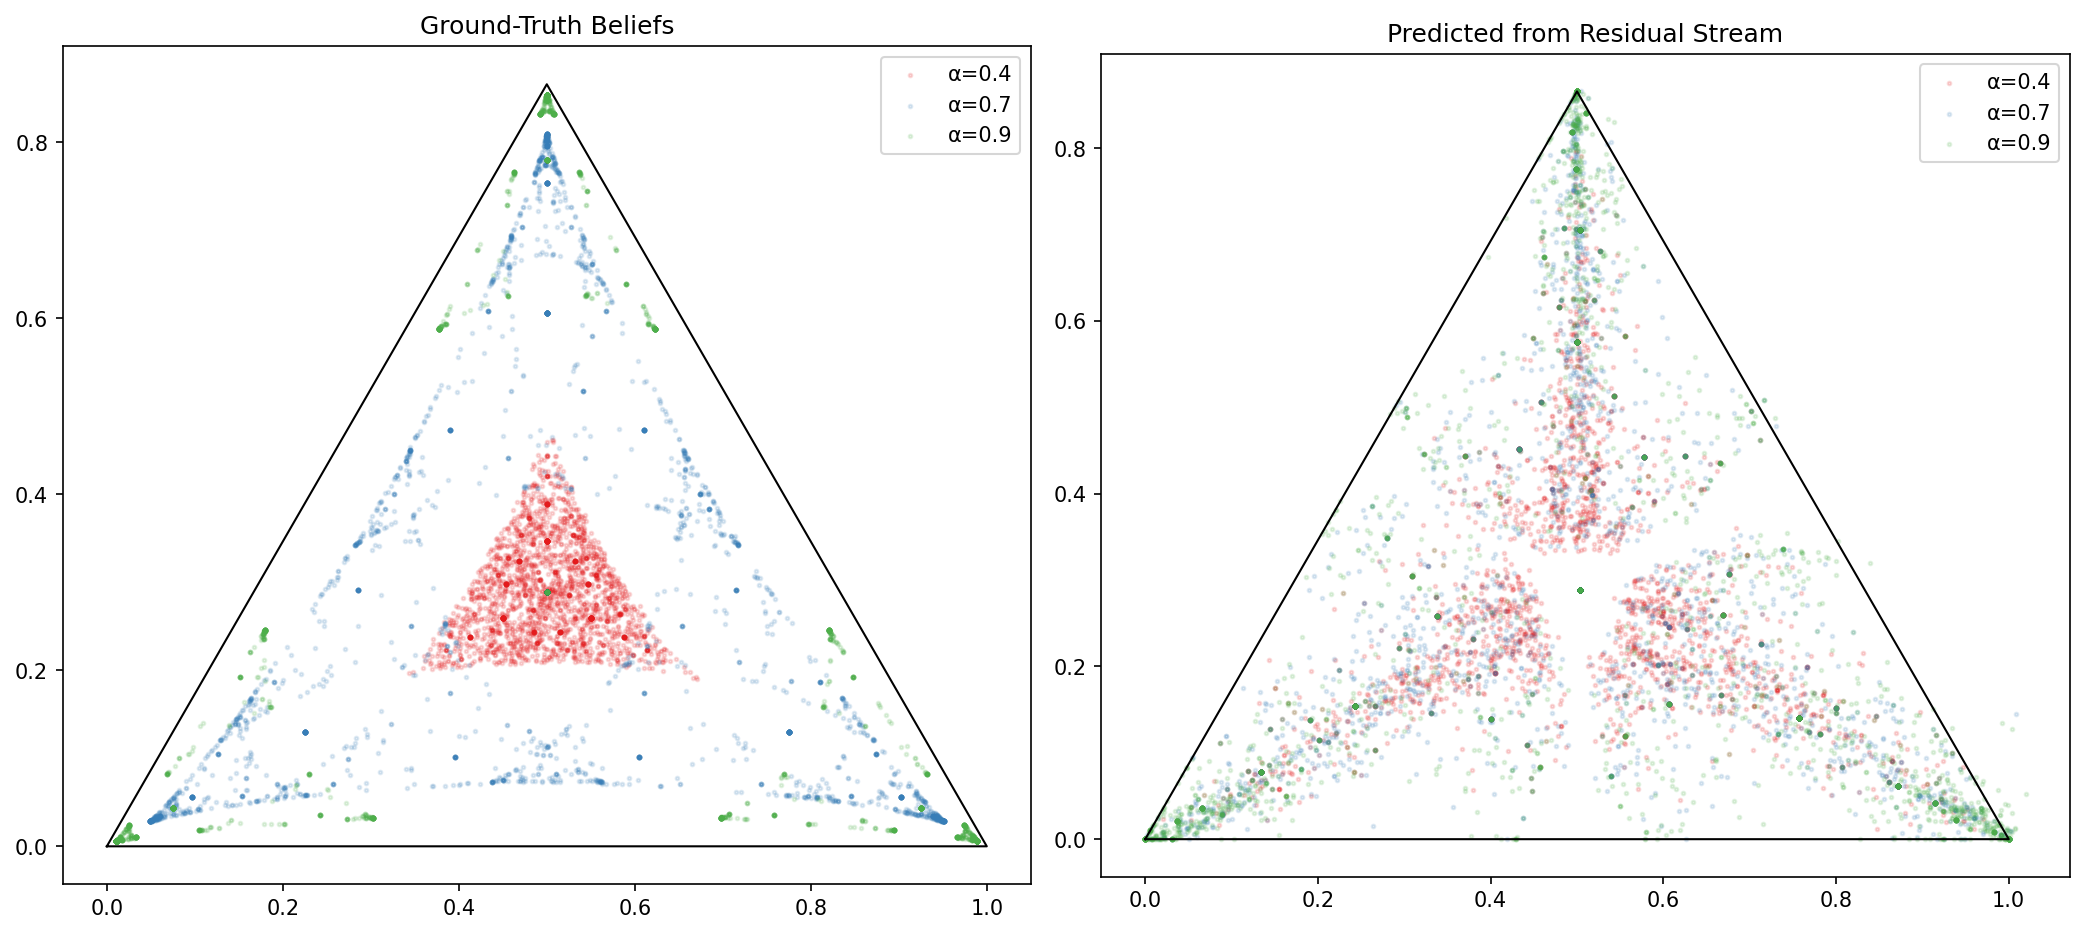
\includegraphics[width=0.9\textwidth]{figures/belief_simplex.png}
  \caption{Ground-truth belief states (left) vs beliefs predicted from the
    residual stream via Ridge regression (right), projected onto the 2-simplex.
    Colors indicate component identity.}
  \label{fig:simplex}
\end{figure}

\begin{figure}[htbp]
  \centering
  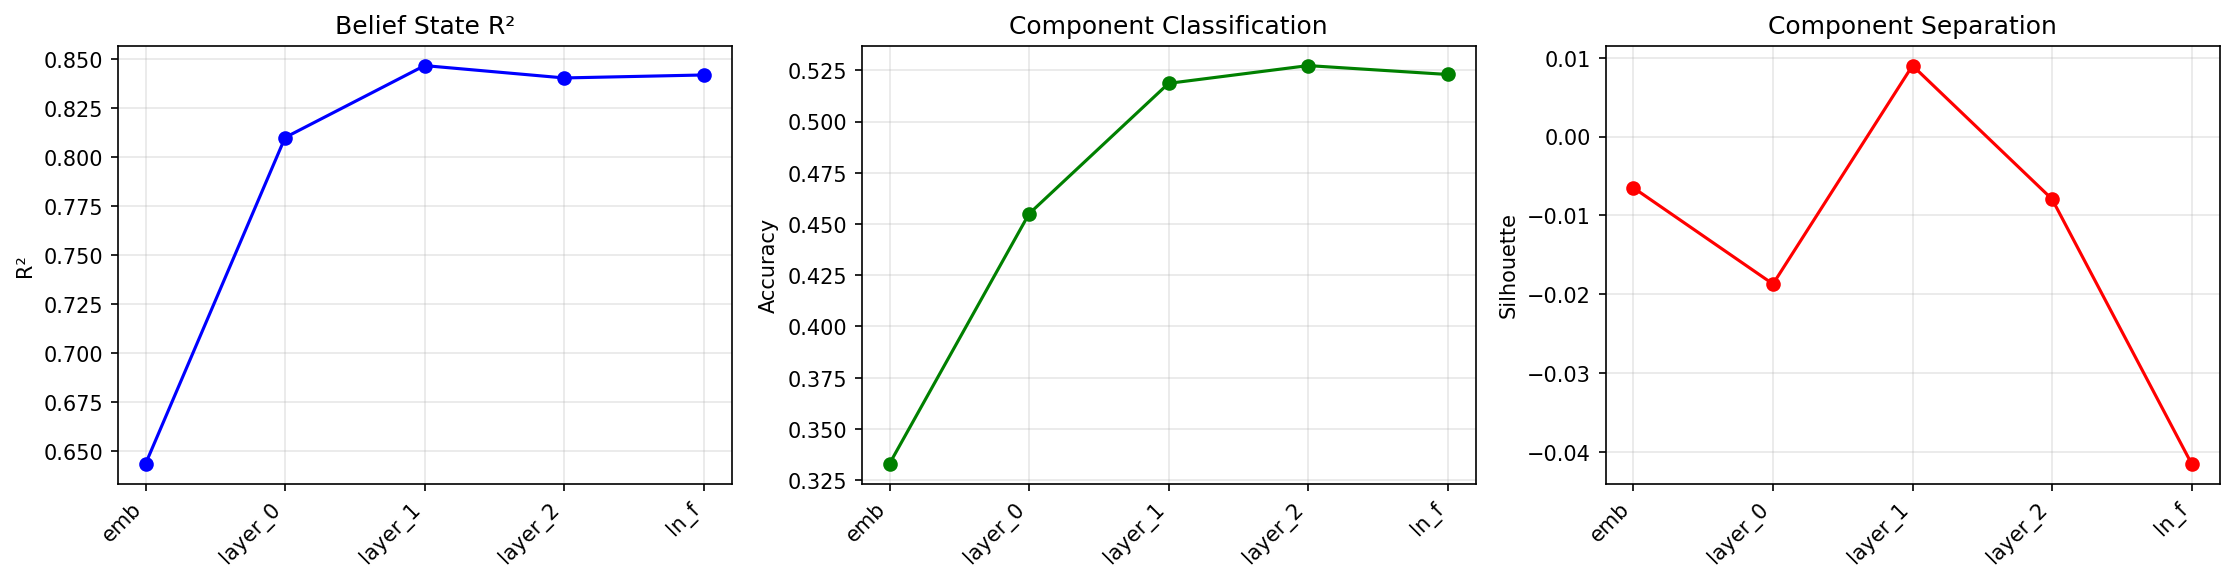
\includegraphics[width=0.9\textwidth]{figures/pred2_layer_metrics.png}
  \caption{Belief $R^2$, component classification accuracy, and silhouette score
    across layers. $R^2$ increases while silhouette remains near zero.}
  \label{fig:layers}
\end{figure}

\begin{figure}[htbp]
  \centering
  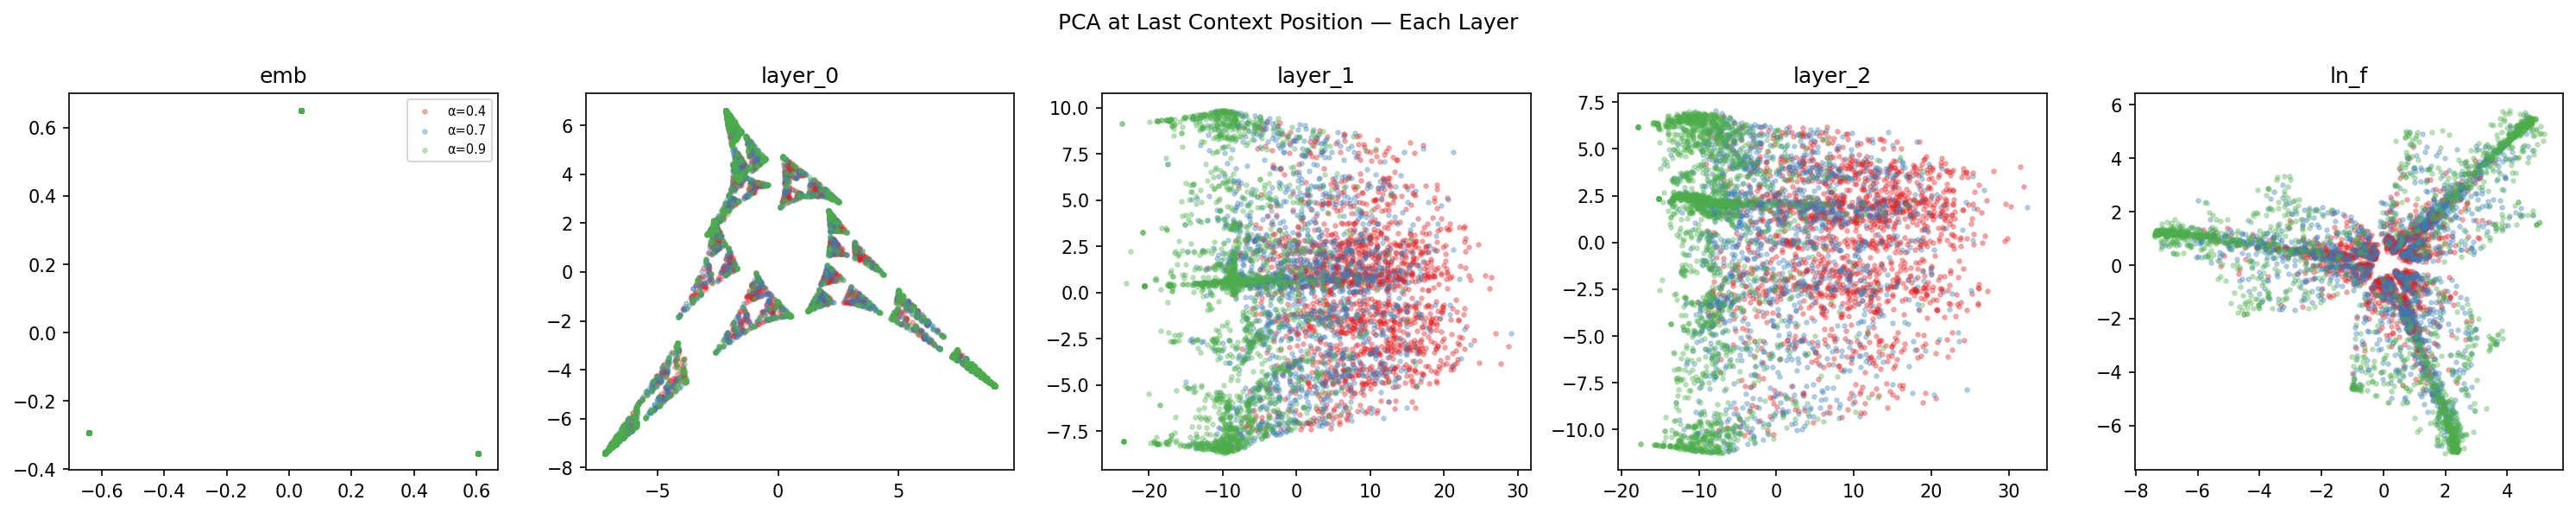
\includegraphics[width=0.9\textwidth]{figures/per_layer_pca.png}
  \caption{PCA at the last context position for each layer. Components overlap
    throughout, confirming the shared-subspace geometry.}
  \label{fig:pca}
\end{figure}

% ------------------------------------------------------------------
\section{Additional Analysis}

% YOUR WRITING HERE
%
% Subsection: Activation Patching
% Activation patching numbers:
%   KL(original || patched) = 0.000
%   KL(patched || target_B) = 0.190
%   Interpretation: patching the belief subspace from component A to B
%   does not change model output, consistent with shared geometry
%
% Subsection: MLP vs Attention Decomposition
% MLP vs attention decomposition numbers:
%   Layer 0: attn R2=0.682, mlp R2=0.795
%   Layer 1: attn R2=0.455, mlp R2=0.781
%   Layer 2: attn R2=0.381, mlp R2=0.742
%   Key finding: MLPs carry more belief info than attention at every layer
%
% Subsection: Bayes-Optimal Baseline (motivated by P2)
%   Compares model per-position CE to oracle CE (Bayesian observer with known component)
%   Shows how close the model gets to theoretical ceiling
%   Metrics: per-position CE gap (model - oracle), overall gap curve
%
% Subsection: Cross-Component Transfer Probes (motivated by P1)
%   Train Ridge probe on alpha_i sequences only, test on alpha_j
%   Produces 3x3 R2 transfer matrix
%   If shared subspace is real, off-diagonal R2 should be close to diagonal
%   Metrics: 3x3 R2 matrix, mean off-diagonal vs diagonal R2
%
% Subsection: OOD Generalization alpha=0.6 (motivated by P1+P2)
%   Generate sequences from unseen alpha=0.6, extract activations
%   Test in-distribution probe on OOD data
%   Metrics: OOD R2 vs in-distribution R2, PCA overlay, simplex projection
%   Tests whether model learned the belief update rule vs memorized 3 alphas

% ------------------------------------------------------------------
\section{What I Would Do Next}

% YOUR WRITING HERE

% ------------------------------------------------------------------
\bibliographystyle{plain}
\bibliography{references}

\end{document}
